% allgem. Dokumentenformat
\documentclass[a4paper,12pt,headsepline]{scrartcl}
%Variablen welche innerhalb der gesamten Arbeit zur Verfügung stehen sollen
\newcommand{\titleDocument}{Bachelor- / Masterarbeit}
\newcommand{\subjectDocument}{im Studiengang <Studiengang>}


% weitere Pakete
% Grafiken aus PNG Dateien einbinden
\usepackage{graphicx}
\usepackage{svg}

% Deutsche Sonderzeichen benutzen 
\usepackage{ngerman}

% deutsche Silbentrennung
\usepackage[ngerman]{babel}

% Eurozeichen einbinden
\usepackage[right]{eurosym}

% Umlaute unter UTF8 nutzen
\usepackage[utf8]{inputenc}

% Zeichenencoding
\usepackage[T1]{fontenc}

\usepackage{lmodern}
\usepackage{fix-cm}

% floatende Bilder ermöglichen
%\usepackage{floatflt}

% mehrseitige Tabellen ermöglichen
\usepackage{longtable}

% Unterstützung für Schriftarten
\newcommand{\changefont}[3]{ 
\fontfamily{#1} \fontseries{#2} \fontshape{#3} \selectfont}

% Packet für Seitenrandabständex und Einstellung für Seitenränder
\usepackage{geometry}
\geometry{left=3.5cm, right=2cm, top=2.5cm, bottom=2cm}

% Paket für Boxen im Text
\usepackage{fancybox}

% bricht lange URLs "schoen" um
\usepackage[hyphens,obeyspaces,spaces]{url}

% Paket für Textfarben
\usepackage{color}

%Paket für todos
\usepackage{todonotes}

% Mathematische Symbole importieren
\usepackage{amssymb}

% auf jeder Seite eine Überschrift (alt, zentriert)
%\pagestyle{headings}

% erzeugt Inhaltsverzeichnis mit Querverweisen zu den Kapiteln (PDF Version)
\usepackage[bookmarksnumbered,pdftitle={\titleDocument},hyperfootnotes=false]{hyperref} 
%\hypersetup{colorlinks, citecolor=red, linkcolor=blue, urlcolor=black}
%\hypersetup{colorlinks, citecolor=black, linkcolor= black, urlcolor=black}

% neue Kopfzeilen mit fancypaket
\usepackage{fancyhdr} %Paket laden
\pagestyle{fancy} %eigener Seitenstil
\fancyhf{} %alle Kopf- und Fußzeilenfelder bereinigen
\fancyhead[L]{\nouppercase{\leftmark}} %Kopfzeile links
\fancyhead[C]{} %zentrierte Kopfzeile
\fancyhead[R]{\thepage} %Kopfzeile rechts
\renewcommand{\headrulewidth}{0.4pt} %obere Trennlinie
%\fancyfoot[C]{\thepage} %Seitennummer
%\renewcommand{\footrulewidth}{0.4pt} %untere Trennlinie

% für Tabellen
\usepackage{array}

% Runde Klammern für Zitate
%\usepackage[numbers,round]{natbib}

% Festlegung Art der Zitierung - Havardmethode: Abkuerzung Autor + Jahr
\bibliographystyle{alphadin}

% Schaltet den zusätzlichen Zwischenraum ab, den LaTeX normalerweise nach einem Satzzeichen einfügt.
\frenchspacing

% Paket für Zeilenabstand
\usepackage{setspace}

% für Bildbezeichner
\usepackage{capt-of}

% für Stichwortverzeichnis
\usepackage{makeidx}

% für Listings
\usepackage{listings}
\lstset{numbers=left, numberstyle=\tiny, numbersep=5pt, keywordstyle=\color{black}\bfseries, stringstyle=\ttfamily,showstringspaces=false,basicstyle=\footnotesize,captionpos=b}
\lstset{language=java}

% Indexerstellung
\makeindex

% Abkürzungsverzeichnis
\usepackage[german]{nomencl}
\let\abbrev\nomenclature

% Abkürzungsverzeichnis LiveTex Version
\renewcommand{\nomname}{Abkürzungsverzeichnis}
\setlength{\nomlabelwidth}{.25\hsize}
\renewcommand{\nomlabel}[1]{#1 \dotfill}
\setlength{\nomitemsep}{-\parsep}
\makenomenclature
%\makeglossary

% Abkürzungsverzeichnis TeTEX Version
% \usepackage[german]{nomencl}
% \makenomenclature
% %\makeglossary
% \renewcommand{\nomname}{Abkürzungsverzeichnis}
% \setlength{\nomlabelwidth}{.25\hsize}
% \renewcommand{\nomlabel}[1]{#1 \dotfill}
% \setlength{\nomitemsep}{-\parsep}

% Disable single lines at the start of a paragraph (Schusterjungen)
\clubpenalty = 10000
% Disable single lines at the end of a paragraph (Hurenkinder)
\widowpenalty = 10000
\displaywidowpenalty = 10000

\begin{document}
% hier werden die Trennvorschläge inkludiert
%hier müssen alle Wörter rein, welche Latex von sich auch nicht korrekt trennt bzw. bei denen man die genaue Trennung vorgeben möchte
\hyphenation{
Film-pro-du-zen-ten
Lux-em-burg
Soft-ware-bau-steins
zeit-in-ten-siv
}

%Schriftart Helvetica
%\changefont{phv}{m}{n}

% Leere Seite am Anfang
\newpage
\thispagestyle{empty} % erzeugt Seite ohne Kopf- / Fusszeile
\section*{ }

% Titelseite %
% das Papierformat zuerst
%\documentclass[a4paper, 11pt]{article}

% deutsche Silbentrennung
%\usepackage[ngerman]{babel}

% wegen deutschen Umlauten
%\usepackage[ansinew]{inputenc}

% hier beginnt das Dokument
%\begin{document}


\thispagestyle{empty}

%\begin{figure}[t]
% \includegraphics[width=0.6\textwidth]{abb/fh_koeln_logo}
%\end{figure}

\begin{figure}[t]
 \centering
 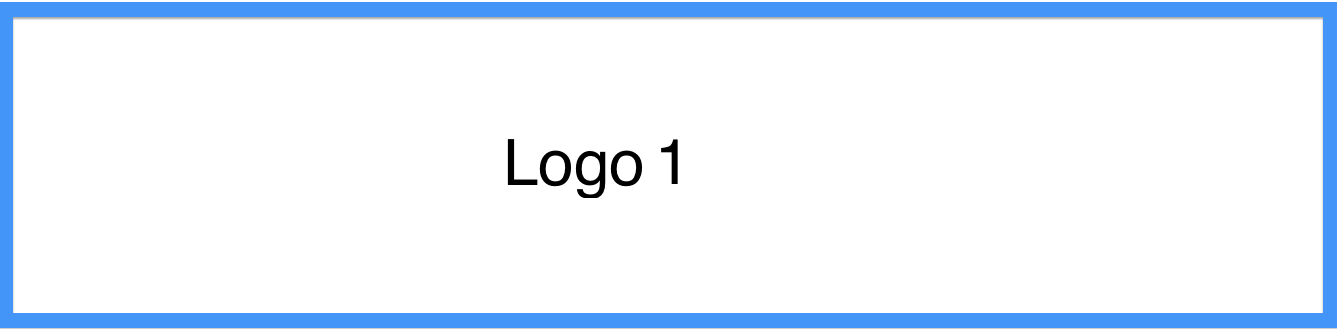
\includegraphics[width=0.6\textwidth]{abb/logo1}
~~~~~~~~~~
 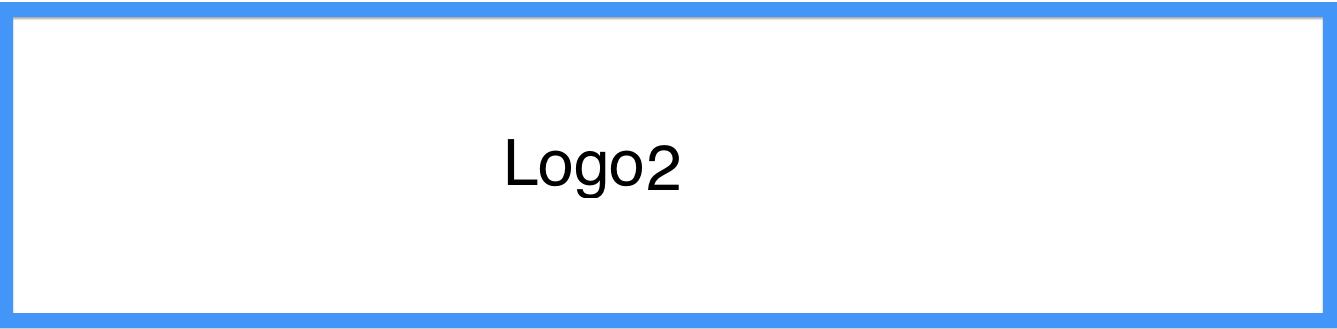
\includegraphics[width=0.3\textwidth]{abb/logo2}
\end{figure}


\begin{verbatim}


\end{verbatim}

\begin{center}
\Large{Fachhochschule <Name>}\\
\Large{- Campus <Name> -}\\
\end{center}


\begin{center}
\Large{Fakultät für <Fachrichtung>}
\end{center}
\begin{verbatim}




\end{verbatim}
\begin{center}
\doublespacing
\textbf{\LARGE{\titleDocument}}\\
\singlespacing
\begin{verbatim}

\end{verbatim}
\textbf{{~\subjectDocument~-~Schwerpunkt <Schwerpunktfach>}}
\end{center}
\begin{verbatim}

\end{verbatim}
\begin{center}

\end{center}
\begin{verbatim}

\end{verbatim}
\begin{center}
\textbf{zur Erlangung des akademischen Grades \\ Bachelor / Master of Science}
\end{center}
\begin{verbatim}






\end{verbatim}
\begin{flushleft}
\begin{tabular}{llll}
\textbf{Thema:} & & <Thema der Arbeit> & \\
& & \\
\textbf{Autor:} & & Name <name@mail.de>& \\
& & MatNr. 12345... & \\
& & \\
\textbf{Version vom:} & & \today &\\
& & \\
\textbf{1. Betreuerin:} & & Prof. Dr. X &\\
\textbf{2. Betreuer:} & & Prof. Dr. Y &\\
\end{tabular}
\end{flushleft}

% römische Numerierung
%\pagenumbering{arabic}

% 1.5 facher Zeilenabstand
\onehalfspacing

% Sperrvermerk
%\section*{Sperrvermerk}
\textcolor{red}{
Die vorliegende Arbeit beinhaltet interne und vertrauliche Informationen der Firma <Firmenname>.
Die Weitergabe des Inhalts der Arbeit im Gesamten oder in Teilen sowie das Anfertigen
von Kopien oder Abschriften - auch in digitaler Form - sind grundsätzlich untersagt.
Ausnahmen bedürfen der schriftlichen Genehmigung der Firma <Firmenname>.
}

% Einleitung / Abstract
\section*{Zusammenfassung}


%\begin{verbatim}

%

%\end{verbatim}




\section*{Abstract}



% einfacher Zeilenabstand
\singlespacing

% Inhaltsverzeichnis anzeigen
\newpage
\tableofcontents

% das Abbildungsverzeichnis
%\newpage
% Abbildungsverzeichnis soll im Inhaltsverzeichnis auftauchen
\addcontentsline{toc}{section}{Abbildungsverzeichnis}
% Abbildungsverzeichnis endgueltig anzeigen
\listoffigures

% das Tabellenverzeichnis
%\newpage
% Abbildungsverzeichnis soll im Inhaltsverzeichnis auftauchen
\addcontentsline{toc}{section}{Tabellenverzeichnis}
% \fancyhead[L]{Abbildungsverzeichnis / Abkürzungsverzeichnis} %Kopfzeile links
% Abbildungsverzeichnis endgueltig anzeigen
\listoftables

%% WORKAROUND für Listings
%\makeatletter% --> De-TeX-FAQ
%\renewcommand*{\lstlistoflistings}{%
%  \begingroup
%    \if@twocolumn
%      \@restonecoltrue\onecolumn
%    \else
%      \@restonecolfalse
%    \fi
%    \lol@heading
%    \setlength{\parskip}{\z@}%
%    \setlength{\parindent}{\z@}%
%    \setlength{\parfillskip}{\z@ \@plus 1fil}%
%    \@starttoc{lol}%
%    \if@restonecol\twocolumn\fi
%  \endgroup
%}
%\makeatother% --> \makeatletter
% das Listingverzeichnis
%\newpage
% Listingverzeichnis soll im Inhaltsverzeichnis auftauchen
\addcontentsline{toc}{section}{Listingverzeichnis}
\fancyhead[L]{Abbildungs- / Tabellen- / Listingverzeichnis} %Kopfzeile links
\renewcommand{\lstlistlistingname}{Listingverzeichnis}
\lstlistoflistings
%%%%

% das Abkürzungsverzeichnis
%\newpage
% Abkürzungsverzeichnis soll im Inhaltsverzeichnis auftauchen
\addcontentsline{toc}{section}{Abkürzungsverzeichnis}
% das Abkürzungsverzeichnis entgültige Ausgeben
\fancyhead[L]{Abkürzungsverzeichnis} %Kopfzeile links
\nomenclature{UGC}{User Generated Content}
\nomenclature{CSS}{Cascading Style Sheets}
\nomenclature{JS}{JavaScript}
\nomenclature{SQL}{Structured Query Language}
\nomenclature{GPL}{GNU General Public License}
\nomenclature{GNU}{GNU is not Unix}
\nomenclature{LGPL}{GNU Lesser General Public License}
\nomenclature{XMPP}{Extensible Messaging and Presence Protocol}
\nomenclature{IM}{Instant Message}
\nomenclature{CMS}{Content Management System}
\nomenclature{RSS}{Really Simple Syndication}
\nomenclature{JSON}{JavaScript Object Notation}
\nomenclature{HTML}{Hypertext Markup Language}
\nomenclature{TDD}{Test-driven development}
\nomenclature{GUI}{Graphical User Interface}
\nomenclature{KPI}{Key Performance Indicator}
\nomenclature{WWW}{World Wide Web}
\nomenclature{OCR}{Optical Character Recognition}
\nomenclature{ERM}{Entity Relationship Modell}

\printnomenclature

% Definiert Stegbreite bei zweispaltigem Layout
\setlength{\columnsep}{25pt}

%%%%%%% EINLEITUNG %%%%%%%%%%%%
%\twocolumn
\newpage
\fancyhead[L]{\nouppercase{\leftmark}} %Kopfzeile links

% 1,5 facher Zeilenabstand
\onehalfspacing

% einzelne Kapitel
\section{Einleitung}\label{1_einleitung}

Mit dem Abschluss einer jeden Berufsausbildung oder eines Studiums beginnt auch der Einstieg in das Berufsleben. Für Viele Bewerber bedeutet das, vermeintlich in Frage kommende Jobangebote zu sichten, und vergleichen. Es folgt das schreiben unzähliger individueller Bewerbungen von denen im schlimmsten Fall nur wenige zu einem Vorstellungsgespräch führen. Doch oftmals kommen schon bereits nach den ersten Wochen des Hochgefühls endlich eine Stelle zu haben, erste Zweifel ob der Job der richtige für einen ist, und die eigenen Wünsche und Anforderungen erfüllen kann.

Auch für Personaler stellt die Einstellung von neuem Personal eine schwierige Aufgabe dar. So müssen oft aus einer Reihe von Bewerbern die tatsächlich unqualifizierten aussortiert werden und eine Auswahl getroffen werden, welche Bewerber zu einem Gespräch eingeladen werden oder in die nächste Bewerbungsrunde gelangen.
 
Es besteht also Bedarf den Prozess von Arbeitsvermittlungen zu optimieren und zu vereinfachen. Das spart sowohl Bewerbern als auch Arbeitgebern viel Frust und Zeit. Ein automatischer Abgleich von Kompetenzen kann diesen Prozess beschleunigen, setzt aber einen einheitlichen Rahmen für die Beschreibung von Kompetenzen voraus. 
 \vspace{1em}
Erlangte Fähigkeiten und Wissen werden im allgemeinen durch Abschlüsse, Zertifikate oder Urkunden bestätigt. Jeder Arbeitnehmer hat einen oder mehrere Abschlüsse die ihn für einen bestimmten Beruf qualifizieren. Leider unterscheiden sich die Bezeichnungen dieser Abschlüsse, beinhalten aber oft dieselben oder ähnliche Kompetenzen. So gibt es neben dem normalen Informatikstudium auch Angebote wie: 
 

\begin{itemize}
  \item Wirtschaftsinformatik
  \item Angewandte Informatik
  \item Medizininformatik
\item Bioinformatik
\item Medieninformatik
\item Technische Informatik
\item Navigation und Umweltrobotik

\end{itemize}

 
Diese Studiengänge haben zwar unterschiedliche Inhalte, bauen aber auf denselben Grundlagen wie zb. Mathematik, Algorithmik, Datenbanken etc. auf. 



Hinführung zum Thema Kompetenzen als Graph Verbindungen Hierachien etc., gibt es Technologie dafür?



\section{Grundlagen und Begrifflichkeiten}\label{2_grundlagen}

%Kompetenzen
%RDF Semantic Web & Linked Data
%Graphen
%Graphentheorie 
%Graphdatenbanken

\subsection{Kompetenzen}\label{competencies}

Im Allgemeinen spricht man bei der Verbindung von Wissen und Können um geforderte Handlungen zu bewältigen von Kompetenzen. Dabei liegt der Fokus auf Fähigkeiten und Wissen, welche dazu beitragen Probleme mit nicht standardmäßigen Handeln zu lösen, und auf verschiedene Situationen zu übertragen.\footnote{vgl. Bundesinstitut für Berufsbildung\cite{bibb}}Oftmals werden die beiden Begriffe Kompetenz und Qualifikation als Synonyme verwendet, jedoch gibt es signifikante Unterschiede in deren Bedeutung.
\vspace{1em}

Kompetenz \footnote{vgl. Bauer 2015\cite{Bauer2015}}(lateinisch: competere, zu etwas fähig sein) meint Lernerfolg im Hinblick auf den Lernenden selbst und seine Befähigung zu selbstverantwortlichem Handeln im privaten, beruflichen und gesellschaftlichen Bereich. Sie bezeichnet die subjektive Leistungsfähigkeit einer Person, welche nicht überprüfbar und objektiv Bewertbar ist.\newline

Qualifikationen\footnote{vgl. Bauer 2015\cite{Bauer2015}} (lateinisch: qualis facere, Beschaffenheit herstellen) sind hingegen prüfbar und Zertifizierbar. Sie sind die äußere Seite der Leistungsanforderung und auf die Erfüllung vorgegebener Zwecke gerichtet. 


\subsection{Kompetenzframeworks}

Kompetenzen abzubilden gestaltet sich schwierig, da diese einen dynamischen Charakter hat um vom Kontext, ihrer Domäne abhängig ist. Durch die Unterteilung in Branchen und Sektoren ist eine Klassifizierung von Kompetenzen dann möglich. Eine weitere Dimension zur Klassifikation ist das Niveau, es beschreibt das Maß oder auch den \emph{Schwierigkeitsgrad} einer Handlung die mit der gegebenen Kompetenz zu bewältigen ist. 
\vspace{1em}

Da Abschlüsse keine Kompetenz bescheinigen, werden Qualifikationsrahmen benötigt, mit deren Hilfe die in einem Bildungsweg erworbenen Kenntnisse und Fähigkeiten zu Kompetenzentwicklung beitragen können. Mit diesen Lernergebnissen die das \emph{Können} im Sinne von \emph{in der Lage sein, etwas zu tun} beschreiben, ergeben sich dann Vergleichsmöglichkeiten.
\vspace{1em}

Um Qualifikationen und Kompetenzen aus unterschiedlichen sektoralen oder nationalen Rahmenwerken zu vergleichen benötigt es einen Meta-Rahmen. 
\vspace{6em}


\subsection{RDF, Semantic Web  Linked Data}\label{semantic_web}
\subsubsection{Semantic Web}
Das Semantic Web stellt Daten, im World Wide Web in einem für Maschinen verarbeitbaren Art und Weise zur Verfügung mit dem Ziel der Interoperabilität, also der Möglichkeit Informationen zwischen Anwendungen und Plattformen auszutauschen und diese in Beziehung zu setzen. Kernaspekte sind das Auffinden relevanter Informationen, die Integration von Informationen aus verschiedenen Quellen und automatische Schlussfolgerung. Die Ziele des Semantik Web lassen sich grob zusammen fassen als Absicht Methoden und Wege zu finden um "Informationen so zu repräsentieren, dass Maschinen damit in einer Art und Weise umgehen können, die aus menschlicher Sicht nützlich und sinnvoll erscheint.”\footnote{ vgl. Hitzler 2007\cite[12]{Hitzler2007}}\newline
 
Im folgenden sollen einige Konzepte und Technologien erläutert werden welche die Anforderungen des Semantic Webs umsetzen.
 
\subsubsection{Linked Data}

Die Beziehungen der Daten im Semantic Web müssen nicht auf ein Datensatz beschränkt bleiben. So können Daten auch Querverweise auf andere Datensätze haben. Ein Beispiel sind die Daten von Wikipedia die durch das Linked Dataset DBPedia zugänglich sind. Einzelne Einträge beinhalten dabei Verweise auf das Geonames Dataset.
Einige dieser Datensätze sind öffentlich zugänglich (Linked Open Data). So stellt das Amt für Veröffentlichungen der Europäischen Union mit ihrem offenen Datenportal Daten ihrer Institutionen und anderer Einrichtungen zur Verfügung. \newline
 
Die Vorgehensweise bei der Erstellung von Linked Data wird von Tim Berners-Lee\footnote{vgl. Bernes-Lee\cite{ld}} in folgenden 4 Schritten beschrieben:

\begin{enumerate}
	\item Dinge und Objekte werden durch URIs identifiziert
	\item Die URIs sind über das HTTP Protokoll aufrufbar
	\item Beim Aufruf werden relevante Informationen in standardisierten Formaten geliefert
	\item Die gelieferten Daten enthalten Referenzen auf andere URIs
\end{enumerate}
\subsubsection{RDF}

Um die Anforderung des Semantic Web’s, Daten im Web auszutauschen, zu erfüllen, wurde das Resource Description Framework RDF als eine formale Sprache für die Beschreibung strukturierter Informationen geschaffen. Dabei soll die ursprüngliche Bedeutung erhalten bleiben und Kombinationen und Weiterbearbeitung der enthaltenen Informationen ermöglicht werden.
Eine Resource kann generell jedes Objekt mit einer eindeutigen Identiät sein, wie zb. Bücher, Orte, Menschen oder abstrakte Konzepte. Um Mehrdeutigkeiten zu verhindern werden URIs als Bezeichner verwendet. Diese RDF-Beschreibungen können auch durch Zeichenketten syntaktisch dargestellt werden, müssen vorher jedoch in Bestandteile zerlegt und serialisiert werden. Die dabei entstehenden Dokumente sind gerichtete Graphen, wobei Knoten und Kanten mit eindeutigen Bezeichnern beschriftet sind. \newline
 
Triple RDF-Graphen lassen sich vollständig durch ihre Kanten beschreiben. Eine solche Kante hat einen Anfangspunkt, eine Beschriftung und einen Endpunkt. Dieses Triple wird bestimmt durch \emph{Subjekt-Prädikat-Objekt}.

\subsubsection{Ontologie/Vokabular}

Als Ontologie oder Vokabular wird eine Sammlung von Begriffen bezeichnet, die innerhalb einer Domäne \textit{Wissen} abbilden und klassifiziert werden.\footnote{What is a Vocabulary?  \cite{w3c}} Mit Hilfe eines Vokabulars werden Regeln über die Semantik von Klassen, Attributen und Beziehungen von Daten definiert. Ontologien können auch in einer spezifischeren Domäne erweitert werden. In der \textit{Simple Knowledge Organization System} Ontologie wird durch die \textit{Concept} Klasse eine Idee oder ein Sachverhalt abgebildet und mit anderen verknüpft. Auch Vererbung und hierarchische Strukturen sind möglich.


\subsection{Graphen}

Ein Graph ist definiert als eine Menge von Knoten (Vertices) und deren Beziehungen, welche über Kanten (Edges) dargestellt werden. Mit Graphen kann man vernetzte Strukturen wie zb. Straßennetze, Computernetzwerke oder Datenstrukturen modellieren. So finden sich in vielen modernen Technologien wie Routenplaner oder Social Media Anwendungen graphentheoretische Konzepte wieder.
	\subsubsection{Graphentheorie}
	Die Graphentheorie is ein Teilgebiet der Mathematik, in dem Graphen und ihre Beziehungen zueinander untersucht. Das älteste dokumentierte Problem der Graphentheorie ist das Königsberger Brückenproblem. Dabei wurde ein Rundweg durch Königsberg gesucht, der alle Brücken jedoch nur einmal überquerte. Leonhard Euler erkannte 1736, dass man die einzelnen Ufer als Punkte und Brücken als Kanten abstrahieren konnte. Euler zeigte, dass ein solcher Weg nicht existierte, da jeder Knoten mit einer ungeraden Anzahl von ungerichteten Kanten verbunden sein muss.
	\newline
	
	Da dieses Themengebiet sehr umfassend ist sollen hier nur einige für diese Arbeit relevante Konzepte erwähnt werden.\newline
	
	\textbf{Gerichteter Graph: }
	
	Ein gerichteter Graph ist definiert als G = (V,R, $\alpha$ , $\omega$) mit V als nicht leere Menge von Knoten, R als Kantenmenge.  $\alpha$ und $\omega$ sind jeweils Abbildungen für die gilt r($\alpha$,$\omega$), wobei r eine Kante ist die ihren Ursprung im Anfangsknoten $\alpha$ hat und im Endknoten $\omega$ endet. \cite[7]{Krumke2012}
	\newline
	
	\textbf{Adjazenmatrix:}
	
	Die Adjazenzmatrix oder auch Nachbarschaftsmatrix ist eine  $n\times n $Matrix mit n = |V|. Sie gibt welche Knoten im Graphen miteinander verbunden sind. Für die Adjazenzmatrix \textit{A(G)} gilt $a_{aj}$ = | \{ $r \in R: \alpha(r) = v_{i}$ und $\omega(r) = v_{j} $ \} |. \cite[17ff]{Krumke2012}\newline	

	\textbf{Gewichtete Kanten:}
	
	Eine Kante kann bewertet werden. Sie wird mit einer Zahl notiert. Diese Zahl kann dann als Parameter verwendet werden und gibt die Kosten an, die anfallen wenn die Kante von einem Algorithmus oder einer Funktion passiert wird.
	\cite[18]{Krumke2012}
	
	
	
	\subsubsection{Graphendatenbanken}	
	Im Gegensatz zu relationalen Datenbanken werden Daten nicht in Tupeln als Tabellen gespeichert sondern als Knoten in einem Graphenmodell. Der Vorteil darin liegt zunächst in der Daten Modelierung, da das Graphen Model sehr intuitive ist und sich einfach auf Papier modelieren lässt. 
	Ein weiterer wichtiger Aspekt ist der Performance Vorteil bei Abfragen von stark verknüpften Daten. Abfragen in relationalen Datenbanken werden langsamer, je größer der Datenbestand. Im Graphen wird immer nur der Teilgraph durchlaufen welcher, die die Abfrage erfüllt.\cite[8]{robinson_webber_eifrem_2015}
	
	\subsubsection{Neo4J}
	
	Die Open Source Graphdatenbank Neo4j ist durch ein \textit{Property Graph Model} implementiert. Knoten im Graph können durch \emph{Label (Beschriftungen)} in Kategorien eingeordnet werden und speichern Informationen in Schlüssel-Wert Paaren als \emph{Properties (Eingeschaften)}. 
	Neben Knoten können auch Kanten Eigenschaften erhalten, was eine Gewichtung der Beziehungen zwischen Knoten ermöglicht, indem man z.B. eine Zahl als Eingeschaft für eine Kante speichert. Eine Beziehung besteht immer aus einem Start- und Endknoten, sowie einer Richtung.\cite[26]{Robinson2015}
	Anfragen an die Neo4j Datenbank werden mittels der deklarativen Sprache \textit{Cypher} ausgeführt. Mit dieser Sprache können Daten gefunden werden, welche einem Muster  entsprechen. Diese Patterns setzen sich aus Knoten und Beziehungen zusammen.\newline
	
%	\begin{figure}[htb]
% \centering
% \includesvg{abb/cypher}
% \caption[Beschreibung]{Cypher mit der Beziehung "mag"}
%\label{fig:Beschreibung}
%\end{figure}

Mit der \textit{MATCH} Klausel, werden alle Pfade im Graphen gezeigt, welche dem Pattern entsprechen. Mit \textit{WHERE} kann die Sammlung gefiltert werden.

\subsection{Empfehlungssysteme}

Ein Empfehlungsystem ist eine Software, welche Nutzern Vorschläge zu Artikeln, Music, Filmen, Büchern oder anderen Objekten macht. \cite{Ricci2010} Ausgehend von einem Objekt werden dem Benutzer andere Objekte mit Ähnlichkeiten zu dem Ausgangsobjekt aufgelistet. Für die Ergebnisse werden im wesentlichen zwei Ansätze verfolgt. Das Inhalts basierte Filtern und Kollaborative Filtern. 
Beim Inhaltsbasierenden Filtern werden Objekte mit einander verglichen. Ein einfacher Anwendungsfall sind zb. Produkt Empfehlungen basierend auf Eigenschaften der Produkte. Wählt ein Benutzer ein Produkt aus, so werden ihm Produkte mit ähnlichen Eigenschaften aufgelistet. 
Mit dem Kollaborativen Filtern wird das Verhalten von Nutzern verglichen. Ein Empfehlungssystem für Online Shops, kann dahingehend erweitert werden, dass nach Produkten gesucht wird die andere Benutzer ebenfalls gekauft haben. 

	

\section{Verwandte Themen und Arbeiten}\label{similar_topics}

\subsection{Openbadge}\label{openbadge}

Auf unserem Bildungsweg werden das Erlangen von Fertigkeiten und Kenntnissen mit Zeugnissen und Abschlüssen belegt. Doch oftmals genügt die formale Ausbildung nicht oder hat aufgrund der sich schnell verändernden Technologien oder Kompetenzen nur eine begrenzte Gültigkeit.  
Die Europäische Union fordert eine stärkere Anerkennung von informalem Lernen, damit auch Fertigkeiten und Kenntnisse die ohne ein formales Abschlusszertifikat erworben wurden Anerkennung finden.\cite{Dorn2014}

Doch wie können Personen alle Ihre Fertigkeiten, welche an einer Hochschule, in einer staatlich Anerkannten Ausbildung oder  in einem Online Seminar, in einem Workshop etc. erworben wurden präsentieren, damit auch Arbeitgeber und Bildungsinstitute in der Lage sind, sicherzustellen, dass Bewerber die nötigen Fertigkeiten mitbringen.\cite{alliance_for_excellent_education}

In der digitalen Welt können sogenannte Badges ein Lösungsansatz sein. Ein digitaler Badge ist ein digitales Zertifikat für eine erbrachte Leistung oder eine Fähigkeit. 
Die Mozilla Foundation hat in Zusammenarbeit mit der MacArthur Foundation den Open Badge(OB) Standard entwickelt. Er stellt sicher, dass Alle Badges Informationen über Kriterien und Nachweise erhalten. Die Informationen in einem Badge können auch auf ein Kompetenzframework verweisen, und validiert werden.\cite[4]{alliance_for_excellent_education}

\vspace{1em}

Badges können von Institutionen, Schulen und Arbeitgebern verliehen werden. Sie definieren ein Set von Kompetenzen oder einen Lehrplan und eine Bewertung um festzustellen ob ein Empfänger die notwendigen Anforderungen erfüllt hat. Darüber hinaus können Badges von ihrem "issuer" mit einer verschlüsselten Zusicherung versehen werden, welche bestätigt, dass der "earner" des Badges die geforderte Leistung auch erbracht hat. 
Die Zusicherung kann dann in den Quellcode eines SVG oder PNG Bildes geschrieben werden, sodass dritte später eine elektronisch Überprüfung beim Herausgeber beantragen können. Über das Alignment-Attribut kann ein Badge auch auf eine Quelle verweisen, welche die Kompetenz oder Fähigkeit beschreibt.

\vspace{1em}
\subsection{Europäischer Qualifikationsrahmen}
Der EQR ist ein Meta-Rahmen, welcher die Vergleichbarkeit von beruflichen Qualifikationen und Kompetenzen aus verschiedenen nationalen oder sektoralen Kompetenzrahmen ermöglichen soll. 
vergleichbarkeit von beruflichen Qualifikationen und Kompetenzen
\subsection{European e-Competence Framework}\label{e-CF}

Der europäische Kompetenzrahmen für Fach- und Führungskräfte der Informations- und Kommunikationstechnologiebranche, ist eine sektor-spezifische Umsetzung des Europäischen Qualifikationsrahmens EQR. Er unterteilt Kompetenzen in 5 Feldern auf 5 Niveaus. 
\subsection{InLoc}\label{inloc}

Das Europäische Projekt InLOC(Integrating Learning Outcomes and Competences) erlaubt es Kompetenzen und Lernergebnisse verschiedener Kompetenzrahmen in einem einheitlichen semantischen Format abzubilden. 


\todo{Wichtig? Mehr Informationen ausarbeiten}

\subsection{ESCO}

In der EU gibt es nach einer Aktuellen Eurostat Statistik ca. 19 Millionen Menschen ohne Beschäftigung. Jedoch haben einige Branchen in Deutschland Probleme Stellen mit qualifiziertem Personal zu besetzen. So blieben im Jahr 2016 In der IT und Telekommunikationsbranche 375.034 Stellen unbesetzt.\cite{Statista2016}
 
Die Europäische Kommission hat dieses Problem erkannt und mit ESCO eine mehrsprachige Klassifizierung für europäische Fähigkeiten, Kompetenzen, Qualifikationen und Berufe entwickelt, deren Zusammenhang durch Berufsprofile verdeutlicht wird.
 
Ein der Aufgaben von ESCO ist es, Die Lücken zwischen dem Arbeitsmarkt und den verschiedenen Bildungssystemen der einzelnen Mitgliedstaaten zu schließen. So unterscheiden sich Qualifikationen welche Menschen in ihren Heimatländern erhalten nicht nur voneinander, sondern können auch oftmals nicht mit aktuellen Entwicklungen des Arbeitsmarktes und dessen Anforderungen mithalten.

Die ESCO Daten werden gemäß den Praktiken für Linked Open Data veröffentlicht. Dies soll Entwicklern den Zugriff erleichtern und Anwendungen für Stellenausgleich, Berufsberatung und Selbsteinschätzungen ermöglichen.

Die Europäische Kommission hat mit ESCO eine Schnittstelle geschaffen, welche Informationen zwischen den nationalen Klassifizierung Systemen übersetzen soll und somit eine höhere semantische Interoperabilität schaffen wird. Ein Hauptinteresse von ESCO ist der kompetenzbasierte Job Abgleich. Arbeitnehmer sollen ihre eigenen Fähigkeiten, Kompetenzen und Qualifikationen mit freien Stellen vergleichen können, und so eventuelle Kompetenzlücken identifizieren zu können. Auf der anderen Seite, muss es Arbeitgebern möglich sein, Stellenausschreibungen durch  Fähigkeiten, Kompetenzen und Qualifikationen zu beschreiben, und Bewerber mit den geforderten Kompetenzen abzugleichen. Diese Anforderungen müssen nun von IT-System erfüllt werden. 


\subsubsection{GraphGist: Recommendation System Sandbox}\label{recommender}

Neo4J bietet über die Sandbox eine interaktive Möglichkeit auf einer temporär generierten Instanz im Browser zu arbeiten. Mit Schritt-für-Schritt Anleitungen werden Themen wie "Netzwerk Management" oder die "Panama Papers" in Neo4j näher gebracht. 

Ein für diese Arbeit relevantes Themenfeld bietet die Sandbox "Recommendations".\cite{neo4j} Als Datenquelle für die Instanz stehen die "Open Movie Database"\cite{omdb}, und das MovieLens Projekt\cite{grouplens_2016} zur Verfügung.
Neben einer Erläuterung zum Property Graph Model und einer Einführung in die Cypher Query Language gibt es Beispiele zu verschiedenen Methoden und Metriken für das Filtern von Ergebnissen. Dabei werden verschiedene Ansätze zu den Methoden Inhaltsbasierte Filterung und Kollaborative Filterung erläutert. 
\subsection{RDF Import Neo4J}

Jesús Barrasa ist  \textit{Senior Graph Solutions Consultant at Neo Technology} bei Neo4j, und hat ein Plugin für Neo4j entworfen, mit dessen Hilfe sich RDF Dokumente in Neo4j importieren lassen. So lässt sich mit dem Befehl :
\vspace{1em}

\begin{lstlisting}[frame=htrbl, caption={Das Listing zeigt einen Funktionsaufruf über die Neo4j}, label={lst:result2}]
CALL semantics.importRDF("file:////..../esco_skos.rdf","RDF/XML",
 { languageFilter: 'de', commitSize: 5000 , nodeCacheSize: 250000})	
\end{lstlisting}

Der komplette RDF Graph des ESCO Kataloges mit allen Beziehungen laden und Abfragen.

%\begin{figure}[htb]
% \centering
% 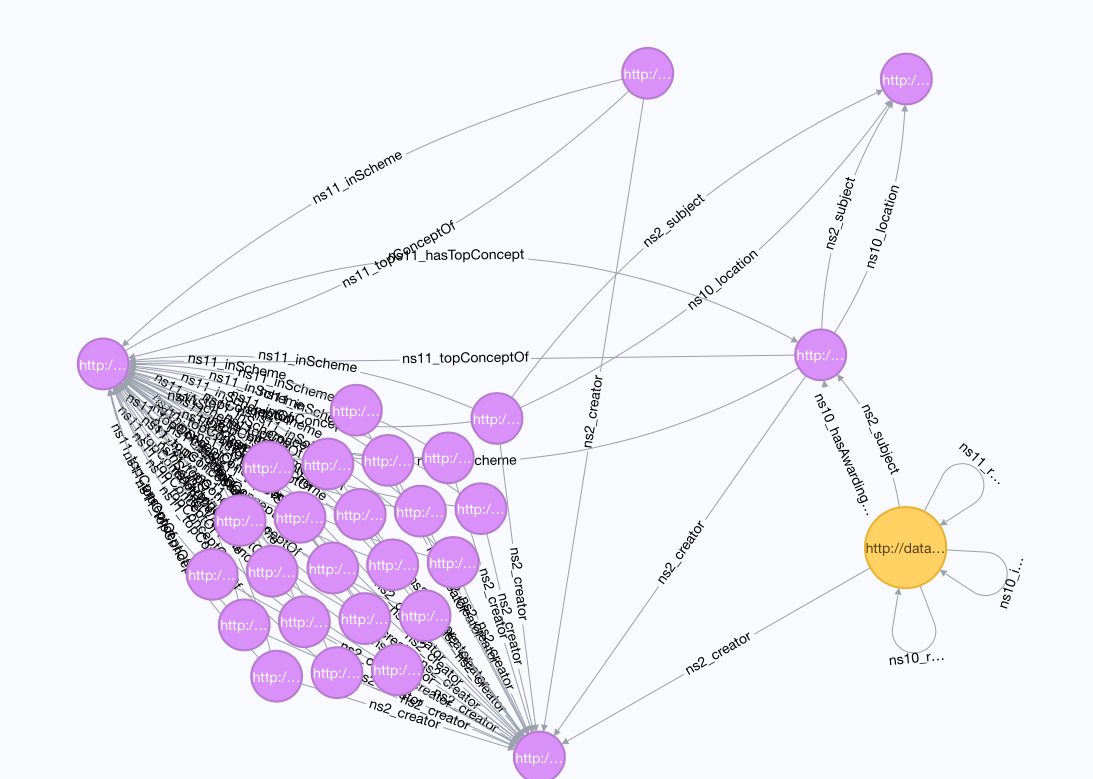
\includegraphics[width=0.3\textwidth,angle=0]{abb/rdf_import_neo4j}
% \caption[Beschreibung]{Beschreibung}
%\label{fig:Beschreibung}
%\end{figure}

\subsection{Recommender Systeme}

Bekannte Anwendungsfälle für ein Recommender System sind neben Musik und Film Empfehlungen vor allem die \textit{andere Kunden kauften auch...} Komponente in Web Shops. Ziel dieser Systeme ist es eine Vorhersage zu treffen, welches Produkt oder Objekt dem Kunden oder Anwender ebenfalls interessieren könnte. Dabei werden häufig die Konzepte des \textit{Inhaltsbasierenden} und des \textit{Kollaborativen} Filtern angewandt. 

Beim Inhaltsbasierten Filtern wird die Ähnlichkeit der Objekte und deren Eigenschaften ermittelt. Im Gegensatz dazu werden beim kollaborativen Filtern Benutzer und deren Präferenzen miteinander verglichen. 


\subsubsection{GraphGist Recommendation Engine Neo4j}

\subsubsection{RecSys Challenge}

Die \textit{ACM RecSys Conference} befasst sich jedes Jahr mit den aktuellen Untersuchungsergebnissen und Techniken im Bereich der Empfehlungsdienste. Darüber hinaus veranstaltet sie auch die RecSys Challenge, einen mit 3000 \euro  Siegerprämie dotierten Wettbewerb, bei dem Teilnehmer ein Empfehlungsdienst, in einer bestimmten Domäne entwickeln sollen. In den beiden vergangen Jahren beschäftigte sich der Wettbewerb mit Job Empfehlungen der Karriereplatform Xing. Die Aufgabe war, anhand eines neuen Job Angebotes, all jene Nutzer zu finden, die interessiert sein könnten eine Benachrichtigung über das neue Angebot zu erhalten aber auch Nutzer die ebenfalls für den Job geeignet sein könnten. Die Ergebnisse werden auf der RecSys Conference in Como, Italien am 27.08.2017 vorgestellt.
\subsubsection{Job-Matching: Xing}

Das Karrierenetzwerk bietet Arbeitssuchenden die Möglichkeit Job-Empfehlungen auf Basis des eigenen Profils zu erhalten. Dabei wird nach den Kriterien Entfernung zum Arbeitsort, Karrierestufe, Skills und Aktivitäten gefiltert. Aus diesen 4 Kriterien wird ein Relevanz-Indikator ermittelt, welcher die Treffgenauigkeit des Inserats angibt. Umgekehrt wird auch ein Inserat mit dem eigenen Profil gematcht, wobei auch die geforderten Skills den eigenen gegenübergestellt werden.\cite{hoelscher}

\begin{figure}[htb]
 \centering
 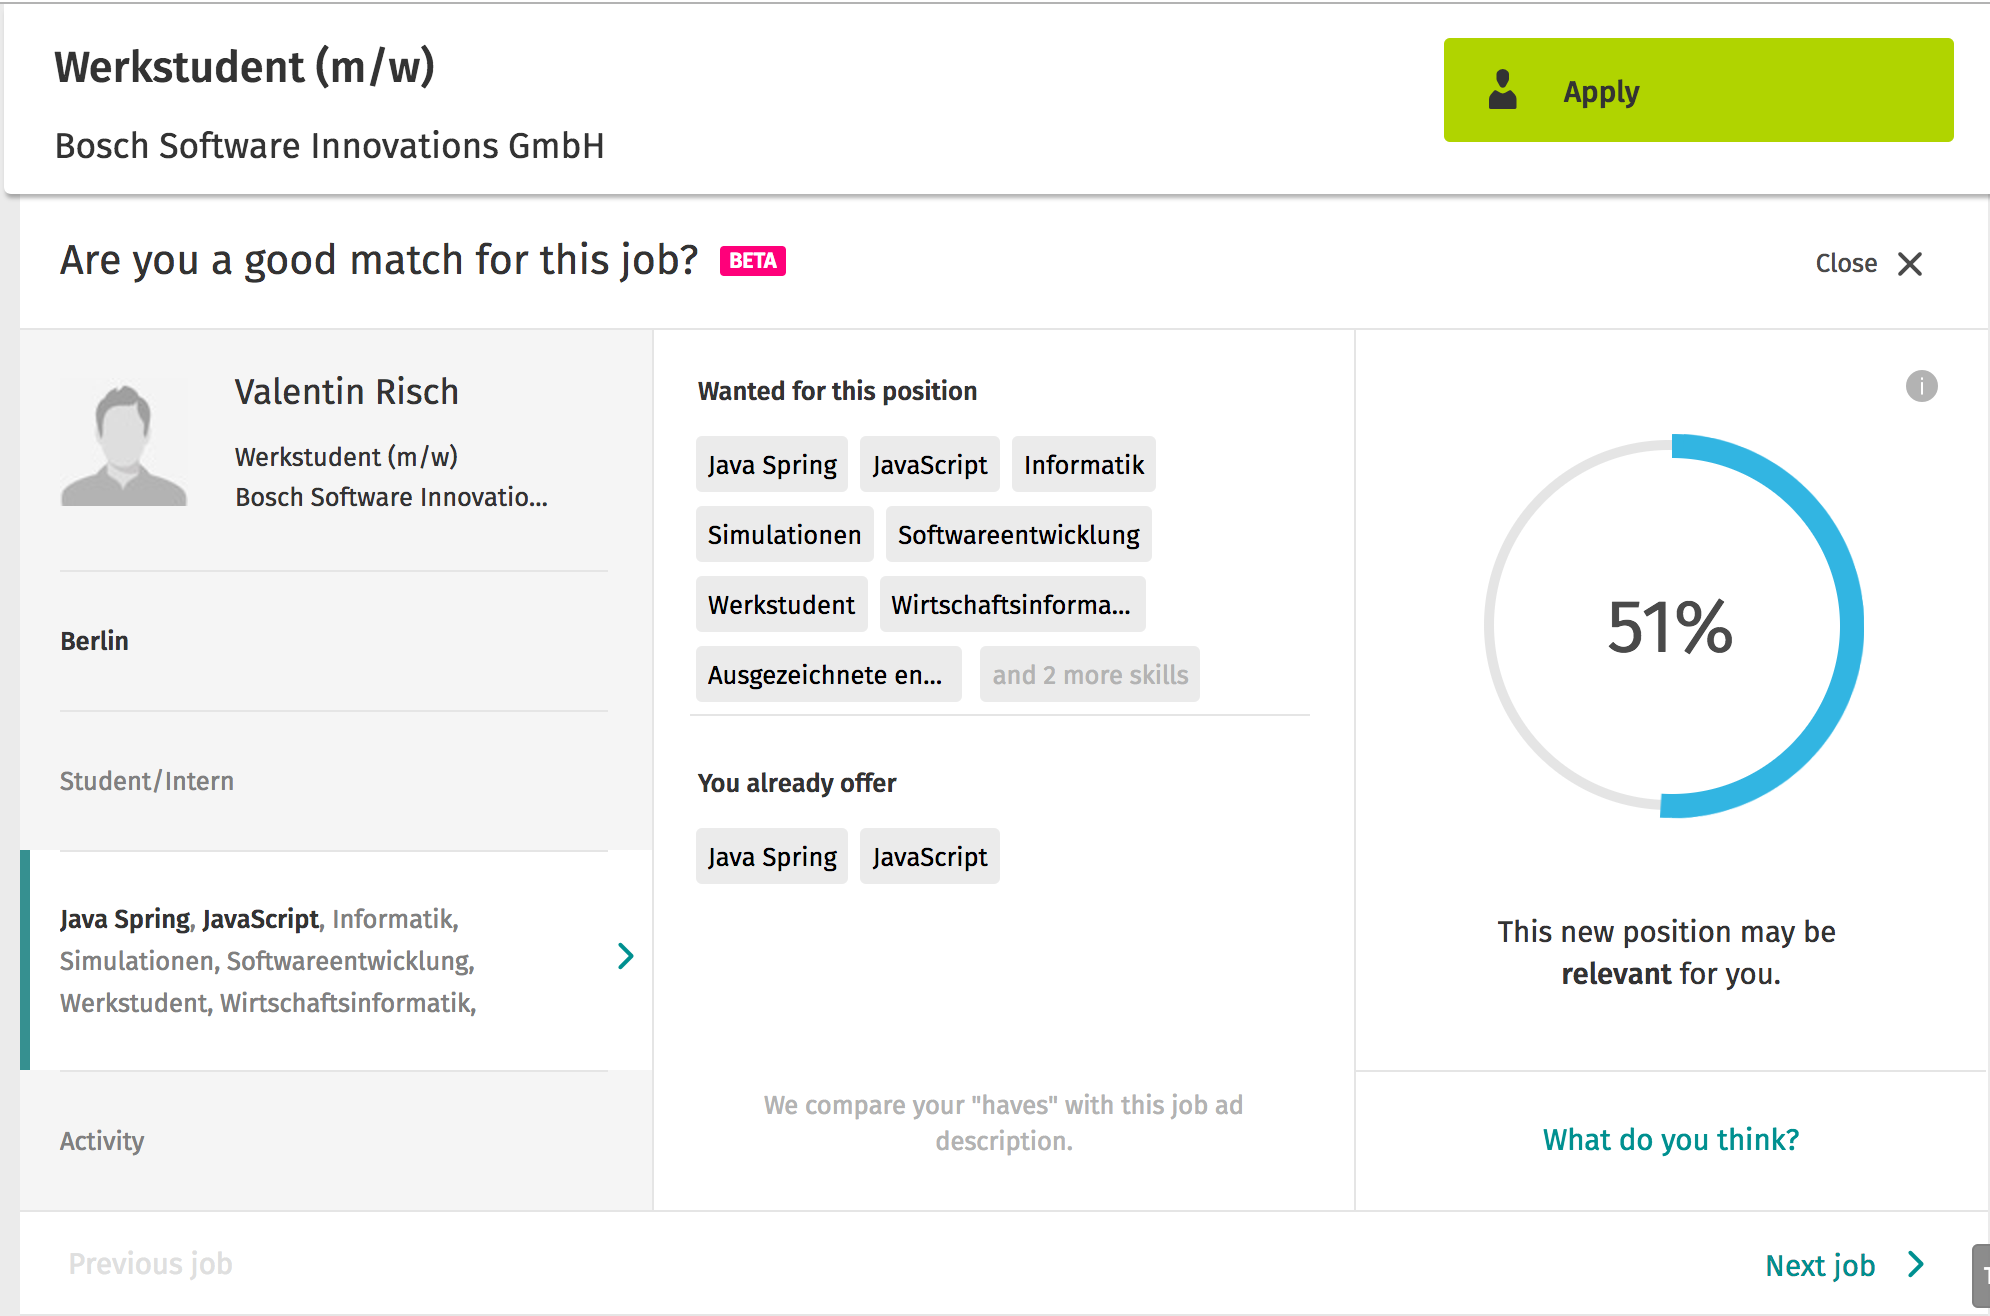
\includegraphics[width=0.7\textwidth,angle=0]{abb/xing_jobmatching}
 \caption[Beschreibung]{Jobmatching Xing-Profil}
\label{fig:Beschreibung}
\end{figure}

Dieser Ansatz berücksichtigt jedoch nicht die Persönlichkeit der Bewerber, und bietet auch nur eine teilweise höhere Bewerberpassgenauigkeit aus Sicht der Arbeitgeber. Wie qualifiziert ein Bewerber wirklich ist bleibt weiter unklar, da eine Liste der angegebenen Skills keine Auskunft darüber gibt wie kompetent der Bewerber auf einem Gebiet wirklich ist. So kann es passieren, dass ein Bewerber der trotz Eignung durch das Raster fällt, weil er andere Schlagworte als die geforderten angegeben hat.

Neben Xing bieten die Plattformen Truffles und BirdieMatch ähnliche Technologien an.






\section{Analyse und Aufgabenstellung}\label{analysis}

Open Badges können über das criteria und alignment field mit Kompetenzen aus externen Kompetenzframeworks verlinkt werden. Daraus ergibt sich die Anforderung Badges mit ähnlichen Kompetezen, Badges die sich ergänzen oder identisch sind zu ermitteln, aber auch fehlende Kompetenzen zu identifizieren die benötigt werden um einen gewünschten Badge zu erlangen. \cite{OBNO3-A2}


Problematisch sind die verschiedenen Standards der einzelnen Kompetenzframeworks. So gibt es nicht nur nationale und sprachliche Unterschiede sondern auch Unterschiede in den veröffentlichen Formaten. Von den bisher veröffentlichten Kompetenzframeworks bietet momentan nur ESCO den Download der Daten in einem maschinenlesbaren Format(CSV, XML, RDF) an. 
\vspace{1em}

\subsection{Aufgabenstellung}

Ein wichtiger Bestandteil von Stellenbeschreibungen sind auch eine Liste von geforderten Kompetenzen. Kompetenzen lassen sich als Graph modellieren, denn oftmals bestehen zwischen ihnen hierarchische Strukturen und Gemeinsamkeiten. Das Ziel dieser Arbeit soll es sein, Die Beziehungen dieser Kompetenzen in einem Graphenmodell zu analysieren, und Methoden und Metriken zu finden mit deren Hilfe es möglich sein wird, Ähnlichkeiten von einzelnen Kompetenzen oder ganzen Kompetenzsets zu ermitteln. Konkret soll ein Dienst entwickelt werden, der von anderen Programmen genutzt, oder in bestehende Systeme integriert werden kann.


\subsection{Anforderungsanalyse} 

\subsubsection{Kompetenzen}

\subsubsection{Anforderungen an die Engine}
Ein solches Empfehlungssystem soll als eigener Dienst fungieren, und über eine API erreichbar sein. Die Eingabe für das Empfehlungssystem soll eine Kompetenz oder eine ein Set von Kompetenzen sein. Kompetenzen werden in einer Datenschicht persistiert, die die gängigen CRUD Datenbankoperationen ermöglicht. Die API leitet die Kompetenzen dann an eine Methode weiter, welche die nötigen Entitäten und deren Beziehungen zurück liefert. Auf resultierenden Datensätzen können weitere Operationen, wie Aggregation oder Sortierung durchgeführt werden und falls weitere Berechnungen oder Operationen nötig sind die mit der Abfragensprache nicht geleistet werden, mit einer einer gängigen Programmiersprache weitere algorithmische Schritte implementieren. Am Ende sollen 0, 1 oder mehrere Kompetenzen in sortierter Reihenfolge an den Aufrufer zurückgeliefert werden.

Folgende Anforderungen können an dieses System gestellt werden.
\begin{itemize}
	\item Übereinstimmung von Kompetenzsets ermitteln
	\item Ähnlichkeit von Kompetenzsets ermitteln
	\item Ähnliche Kompetenzen finden
	\item Inkludierende Kompetenzen ermitteln
	\item Fehlende von Kompetenzen finden
\end{itemize}

Optionale Anforderungen

\begin{itemize}
	\item Vergleich von Kompetenzen aus verschiedenen Frameworks
\end{itemize}


Mit der Übereinstimmung von Kompetenzsets zb. das einer Stellenbeschreibung und das eines Lebenslaufes, kann ein Matching vorgenommen werden, welches Computersystemen ermöglicht passende Stellenangebote oder Bewerber zu finden. Über die Vernetzung der Kompetenzen im Graphen können Wege zur weiteren Bildung ermittelt werden.


\subsubsection{Anforderungen an die Architektur}

Der Dienst soll als nach dem Microservice Muster implementiert werden, also bei Bedarf komplett austauschbar sein und wenige Abhängigkeiten enthalten. Nutzer sollen über das HTTP Protokoll mit dem Dienst kommunizieren können. Die Daten werden in einem Graphen persistiert, in welchem Kompetenzen als Knoten und Beziehungen der Kompetenzen als Kanten gespeichert werden. Für die Kommunikation soll ein gängiges Format zur Ein und Ausgabe gewählt werden.

\begin{itemize}
	\item Erreichbarkeit über eine Web-API 
	\item Persistenz der Daten in einem Graphen	
	\item Daten Ein und Ausgabe in einem standardisierten Format 
\end{itemize}





\section{Entwurf}\label{entwurf}
\subsection{Format/Kompotenzmodell}

Für die Modellierung der Kompetenzen gibt es mehrere Möglichkeiten. 

\subsubsection{ESCO RDF Import}

ESCO steht als RDF Graph zur mit einem eigenen Vokabular zur Verfügung und kann mittels RDF Importer\todo{Jesus Barrasa zitieren} in die Neo4j Instanz geladen werden. Dabei werden nach den ESCO Ontologien folgende interessante Knoten und Beziehungstypen angelegt. 

ESCO concepts Relationship

IRI: http://data.europa.eu/esco/modelRelationship


Beziehung zwischen zwei ESCO Säulen tb. Occupation und Qualification.

Qualification 

IRI: http://data.europa.eu/esco/modelQualification

Ein offiziell oder formelles Zertifikat eines oder mehrerer Kompetenzen oder Fertigkeiten.

Kann verknüpft im Skills oder Berufen sein.

Skil 

IRI: http://data.europa.eu/esco/modelSkill


\todo{weitere auf https://ec.europa.eu/esco/resources/data/static/model/html/model.xhtml }

\subsubsection{inLOC}

Das Projekt InLOC ermöglicht das Abbilden von allen Kompetenzrahmen in einem einheitlichen maschienenlesbaren Format(RDF,XML,JSON-LD).


\subsubsection{Datenbank}

Für die Persistenz der Kompetenz Daten wird eine Instanz des Neo4j Datenbank Management Systems eingesetzt. Die Vorteile 

Alternative Datenbanken
Warum keine RDF Technologie?
\subsubsection{API}

 Die Funktionsweise der Recommendation Engine soll sich lediglich auf folgende Prozesse beschränken:
 
 Eingabe und Ausgabe einer Kompetenz
Berechnung von Ähnlichkeiten im Graphen durch Graph Traversierung

Die Anwendung ist also wenig Komplex. Ein viel höherer Implementierungsaufwand ist den Vergleichsalgorithmen, bzw Graph Queries zuzurechnen. Um den Implementierungsaufwand der Applikation weiter zu reduzieren, soll das Serverless Framework für Amazon Web Services Lambda zum Einsatz kommen. 

Für die erste Komponente wird eine Web Api benötigt, über welche  mit einem Internetfähigen Protokoll wie zb. HTTP zugegriffen werden kann. 

Die Zweite Komponente muss eine Datenbankanbindung für die Datenbank gewährleisten, und Daten aus der Eingabe in Anfragen an die Datenbank verarbeiten, sowie Ergebnisse der Anfragen zurückliefern. Falls die Anfragensprache der Datenbank nicht alle Möglichkeiten ausschöpfen kann die Ergebnisse wie gewünscht zu filtern, können in der zweiten Komponente weitere Algorithmen implementiert werden.


\begin{figure}[htb]
 \centering
 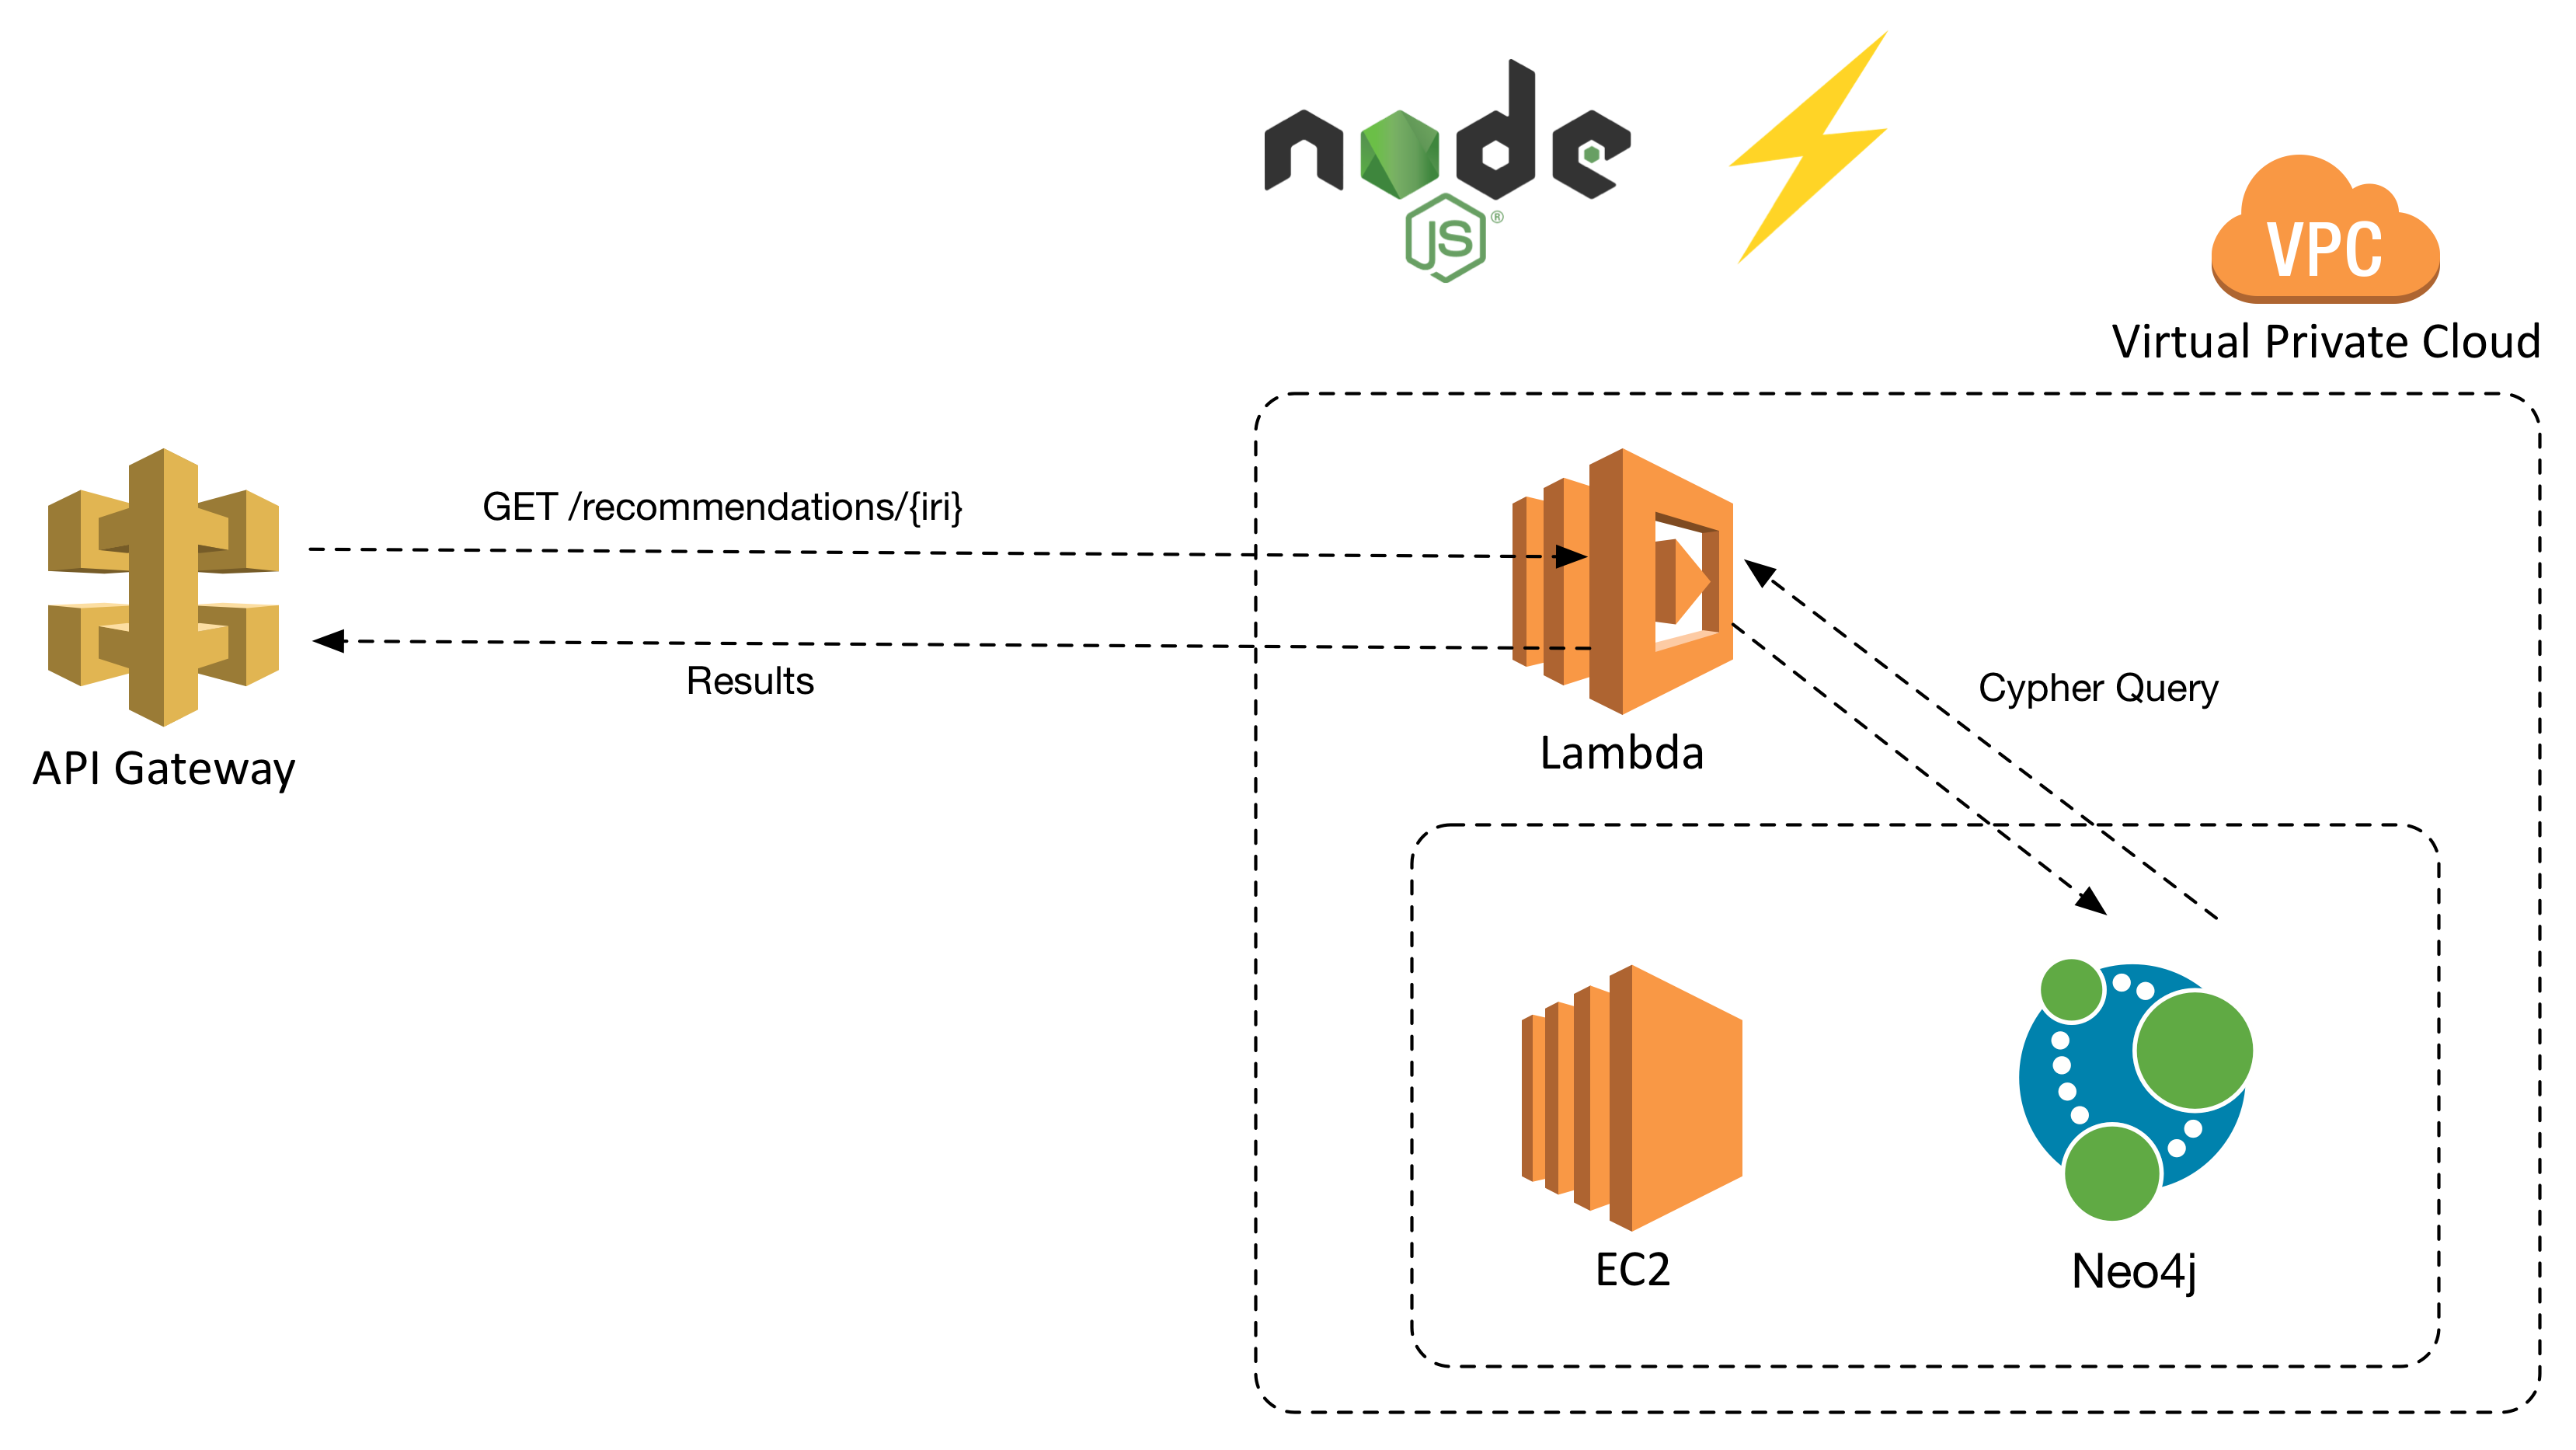
\includegraphics[width=0.7\textwidth,angle=0]{abb/Architecture}
 \caption[Beschreibung]{Beschreibung}
\label{fig:Beschreibung}
\end{figure}

\subsection{Datenmodell}
\subsection{Anfragen Formulieren}
\subsection{Algorithmen}

Shortest Path
Dijkstra Algorithm
Depth First
Breadth first search


\input{6_evaluation}

\section{Ausblick}\label{ausblick}

Der Prototyp des Empfehlungsdienstes ist in seinen Grundzügen fertig implementiert, kann und soll erweitert und verbessert werden. So können weitere Daten mit Kompetenzen in die Datenbank geladen werden, oder neue Beziehungen eingeführt. Eine wichtige Eigenschaft des Neo4j \textit{Label Property Graph} Models, die Gewichtung von Kanten, wird bisher noch nicht genutzt. Der Europäische Qualifikationsrahmen sieht aber Niveau Levels vor, mit diesen könnte sich die Kosinus Ähnlichkeit als weitere Metrik berechnen lassen. 
Die implementierten Methoden zur Ähnlichkeitsmessung sind lediglich ein Ansatz, für einen Vollfunktions umfänglichen Empfehlungsdienst müssten die einzelnen Metriken evaluiert und gegebenenfalls angepasst werden. Im Idealfall werden diese nicht nur einzeln angewandt, sondern mit einander kombiniert. 

  Zum Zeitpunkt der Entscheidung die Daten von ESCO zu verwenden lagen standen diese nur in einer frühen Version 0.8 zur Verfügung. Seit dem 28.07.2017 sind die Daten nun in überarbeiteter Struktur verfügbar und es wurden zb. für die Informations und Technologie Branche relevante Sektor spezifische Kompetenzen hinzugefügt. 

\section{Fazit}\label{fazit}

\begin{figure}[htb]
 \centering

 \caption[Beispiel einer Bildbeschreibung]{Beispiel einer Bildbeschreibung\footnotemark}
\label{fig:beispiel1}
\end{figure}
\footnotetext{Bildquelle: Beispielquelle}

% Beispiel für Bildintegration
\begin{figure}[htb]
 \centering
 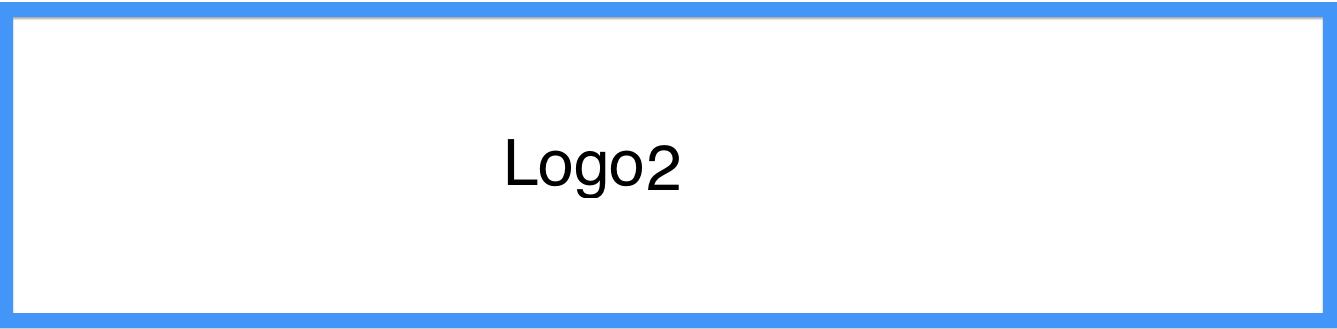
\includegraphics[width=0.3\textwidth,angle=0]{abb/logo2}
 \caption[Beschreibung]{Beschreibung}
\label{fig:Beschreibung}
\end{figure}

% Beispiel: Referenz auf Abbildung
Abbildung~\ref{fig:Beschreibung} [S.\pageref{fig:Beschreibung}]

% Beispiel: Tabelle 
\begin{center}
  \begin{tabular}{ | l | c | }
    \hline
    Überschrift 1 & Überschrift 2 \\ \hline \hline
    Info 1 & Info 2 \\ \hline
    Info 3 & Info 4 \\
    \hline
  \end{tabular}
\end{center}


% Beispiel für Quellcode Listings
\lstset{language=xml}
\lstset{language=java}
\begin{lstlisting}[frame=htrbl, caption={Das Listing zeigt Java Quellcode}, label={lst:result2}]
/* generate TagCloud */
Cloud cloud = new Cloud();
cloud.setMaxWeight(_maxSizeOfText);
cloud.setMinWeight(_minSizeOfText);
cloud.setTagCase(Case.LOWER);
	    
/* evaluate context and find additional stopwords */
String query = getContextQuery(_context);
List<String> contextStoplist = new ArrayList<String>();
contextStoplist = getStopwordsFromDB(query);
	    
/* append context stoplist */
while(contextStoplist != null && !contextStoplist.isEmpty())
  _stoplist.add(contextStoplist.remove(0));
	    
/* add cloud filters */
if (_stoplist != null) {
  DictionaryFilter df = new DictionaryFilter(_stoplist);
  cloud.addInputFilter(df);
}
/* remove empty tags */
NonNullFilter<Tag> nnf = new NonNullFilter<Tag>();
cloud.addInputFilter(nnf);

/* set minimum tag length */
MinLengthFilter mlf = new MinLengthFilter(_minTagLength);
cloud.addInputFilter(mlf);

/* add taglist to tagcloud */
cloud.addText(_taglist);

/* set number of shown tags */	    
cloud.setMaxTagsToDisplay(_tagsToDisplay);
\end{lstlisting}


% Beispiel für Formeln
Die Zuordnung aller möglichen Werte, welche eine Zufallsvariable annehmen kann nennt man \emph{Verteilungsfunktion} von $X$.

\begin{quotation}
Die Funktion F: $\mathbb{R} \rightarrow$ [0,1] mit $F(t) = P (X \le t)$ heißt Verteilungsfunktion von $X$.\footnote{Konen, vgl.~\cite{wk05}~[S.55]}
\end{quotation}

\begin{quotation}
Für eine stetige ABC $X: \Omega \rightarrow \mathbb{R}$ heißt eine integrierbare, nichtnegative reelle Funktion $w: \mathbb{R} \rightarrow \mathbb{R}$ mit $F(x) = P(X \le x) = \int_{-\infty}^{x} w(t)dt$ die \emph{Dichte} oder \emph{Wahrscheinlichkeitsdichte} der Zufallsvariablen $X$.\footnote{Konen, vgl.~\cite{wk05}~[S.56]}
\end{quotation}


\onecolumn
% einfacher Zeilenabstand
\singlespacing
% Literaturliste soll im Inhaltsverzeichnis auftauchen
\newpage
\addcontentsline{toc}{section}{Literaturverzeichnis}
% Literaturverzeichnis anzeigen
\renewcommand\refname{Literaturverzeichnis}
\bibliography{Hauptdatei}
\bibliographystyle{alphadin}

%% Index soll Stichwortverzeichnis heissen
% \newpage
% % Stichwortverzeichnis soll im Inhaltsverzeichnis auftauchen
% \addcontentsline{toc}{section}{Stichwortverzeichnis}
% \renewcommand{\indexname}{Stichwortverzeichnis}
% % Stichwortverzeichnis endgueltig anzeigen
% \printindex

\onehalfspacing
% evtl. Anhang
\newpage
\addcontentsline{toc}{section}{Anhang}
\fancyhead[L]{Anhang} %Kopfzeile links
\subsection*{Anhang}\label{anhang}

\subsubsection{API Endpunkte}



% Eidesstattliche Erklärung
\addcontentsline{toc}{section}{Eidesstattliche Erklärung}
\section*{Eidesstattliche Erklärung}
\thispagestyle{empty}

\begin{verbatim}

\end{verbatim}

\begin{LARGE}Eidesstattliche Erklärung zur <-Arbeit>\end{LARGE}
\begin{verbatim}


\end{verbatim}
Ich versichere, die von mir vorgelegte Arbeit selbstständig verfasst zu haben. Alle Stellen, die wörtlich oder sinngemäß aus veröffentlichten oder nicht veröffentlichten Arbeiten anderer entnommen sind, habe ich als entnommen kenntlich gemacht. Sämtliche Quellen und Hilfsmittel, die ich für die Arbeit benutzt habe, sind angegeben. Die Arbeit hat mit gleichem Inhalt bzw. in wesentlichen Teilen noch keiner anderen Prüfungsbehörde vorgelegen.



\begin{displaymath}
% use packages: array
\begin{array}{ll}
Unterschrift:~~~~~~~~~~~~~~~~~~~~~~~~~~~~~~~~~~~~~~~~~~
& Ort, Datum:~~~~~~~~~~~~~~~~~~~~~~~~~~~~~~~~~~~~~~~~~~
\end{array}
\end{displaymath}


% leere Abschlussseite
\newpage
\thispagestyle{empty} % erzeugt Seite ohne Kopf- / Fusszeile
\section*{ }

\end{document}